\section{Uvod}

\subsection{Uporabna matematika}

\begin{enumerate}[label=\alph*)]
    \item Zgodovinsko (od Newtona in Leibniza):
    \begin{itemize}
        \item temelji na \underline{zvezno spreminjajočih se procesih},
        \item motivirani predvsem z fizikalnimi aplikacijami,
        \item in študiranih z uporabo \underline{analize} (diferencialni račun, integralni račun).
    \end{itemize}    
    \item Z rastjo računalnikov in drugih digitalnih naprav:
    \begin{itemize}
        \item \underline{diskretna matematika} postaja vse pomembnejša.
        \item diskretna matematika študira končne ali števno neskončne diskretne objekte
        \item Zajema številna področja matematike: 
        \begin{itemize}
            \item teorijo množic, 
            \item logiko, 
            \item kombinatoriko, 
            \item teorijo grafov, 
            \item teoretično računalništvo, 
            \item teorijo števil, 
            \item pa tudi (vsaj delno): 
            \begin{itemize}
                \item algebro, 
                \item operacijske raziskave, 
                \item terijo iger, 
                \item verjetnost, 
                \item statistiko.
            \end{itemize}
        \end{itemize}
    \end{itemize}
\end{enumerate}

\subsection{Uporaba diskretne matematike v resničnem življenju}

\begin{itemize}
    \item organizacija sestankov,
    \item sestavljanje proizvodnih in šolskih urnikov,
    \item kriptografija,
    \item načrtovanje kod,
    \item oblikovanje prometnih, električnih in komunikacijskih omrežij,
    \item dodeljevanje zaposlenih na delovna mesta,
    \item oblikovanje glasovnih shem,
    \item načrtovanje poskusov (npr.: Recimo da imate kmetijo, pa želite preiskusit različna gnoila za zemljo, imate na voljo samo 3 njive, pa 7 različnih gnojil, kako jih boste zdej preiskusili katero je boljše. In potem lahko razvijete načrt kako boste to naredili na nek pošten način)
\end{itemize}

\begin{center}

    % fanova ravnina graf
\begin{figure}[H]
    \centering
    \tikzset{every picture/.style={line width=0.75pt}} %set default line width to 0.75pt        

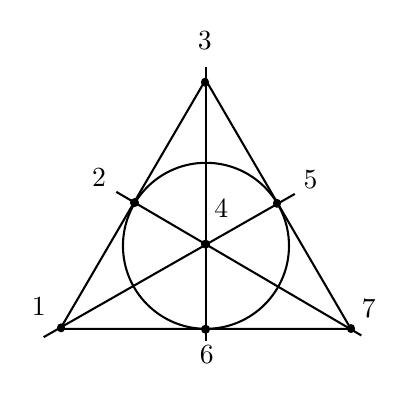
\begin{tikzpicture}[x=0.75pt,y=0.75pt,yscale=-1,xscale=1]
%uncomment if require: \path (0,300); %set diagram left start at 0, and has height of 300

%Shape: Triangle [id:dp3256490994156913] 
\draw   (320.23,70.6) -- (390.2,190.6) -- (250.2,190.6) -- cycle ;
%Shape: Circle [id:dp14206240130920134] 
\draw   (280.4,150.6) .. controls (280.4,128.51) and (298.31,110.6) .. (320.4,110.6) .. controls (342.49,110.6) and (360.4,128.51) .. (360.4,150.6) .. controls (360.4,172.69) and (342.49,190.6) .. (320.4,190.6) .. controls (298.31,190.6) and (280.4,172.69) .. (280.4,150.6) -- cycle ;
%Straight Lines [id:da00745294776731642] 
\draw    (242.2,194.6) -- (363.2,125.6) ;
%Straight Lines [id:da2762334561765414] 
\draw    (277.2,124.6) -- (395.24,193.77) ;
%Straight Lines [id:da4437084246675649] 
\draw    (320.2,64.6) -- (320.2,196.6) ;
%Shape: Free Drawing [id:dp8632448061158087] 
\draw  [line width=3] [line join = round][line cap = round] (319.91,71.96) .. controls (319.79,71.96) and (319.91,71.51) .. (319.91,71.63) ;
%Shape: Free Drawing [id:dp4175873757531443] 
\draw  [line width=3] [line join = round][line cap = round] (390.24,190.63) .. controls (390.13,190.63) and (390.24,190.18) .. (390.24,190.29) ;
%Shape: Free Drawing [id:dp4320796965233138] 
\draw  [line width=3] [line join = round][line cap = round] (320.24,190.96) .. controls (320.13,190.96) and (320.24,190.51) .. (320.24,190.63) ;
%Shape: Free Drawing [id:dp7337895225898607] 
\draw  [line width=3] [line join = round][line cap = round] (250.57,190.29) .. controls (250.46,190.29) and (250.57,189.85) .. (250.57,189.96) ;
%Shape: Free Drawing [id:dp09943922881641676] 
\draw  [line width=3] [line join = round][line cap = round] (354.57,130.29) .. controls (354.46,130.29) and (354.57,129.85) .. (354.57,129.96) ;
%Shape: Free Drawing [id:dp32779299451833666] 
\draw  [line width=3] [line join = round][line cap = round] (285.91,129.96) .. controls (285.79,129.96) and (285.91,129.51) .. (285.91,129.63) ;
%Shape: Free Drawing [id:dp565300018291063] 
\draw  [line width=3] [line join = round][line cap = round] (320.24,149.96) .. controls (320.13,149.96) and (320.24,149.51) .. (320.24,149.63) ;

% Text Node
\draw (235,174) node [anchor=north west][inner sep=0.75pt]   [align=left] {1};
% Text Node
\draw (394,175) node [anchor=north west][inner sep=0.75pt]   [align=left] {7};
% Text Node
\draw (323,127) node [anchor=north west][inner sep=0.75pt]   [align=left] {4};
% Text Node
\draw (366,113) node [anchor=north west][inner sep=0.75pt]   [align=left] {5};
% Text Node
\draw (315,46) node [anchor=north west][inner sep=0.75pt]   [align=left] {3};
% Text Node
\draw (264,112) node [anchor=north west][inner sep=0.75pt]   [align=left] {2};
% Text Node
\draw (316,197) node [anchor=north west][inner sep=0.75pt]   [align=left] {6};


\end{tikzpicture}
\caption{Fanova ravnina}

\end{figure}

\end{center}
\begin{itemize}
    \item v kemiji in \underline{biologiji} (lasti bioinformatiki, v študiju sekvence DNA in filogenetiki),
    \item v razvedrilnih matematiki (Sudoku, Rubikova kocka, Hanoijski stolpi\dots)
\end{itemize}
Pri tem predmetu bomo obravnavali kombinatoriko pa teorijo grafov:
\begin{itemize}
    \item reševanje problemov
    \item dokazovanje
\end{itemize}

\subsection{Kaj je kombinatorika?}
Kombinatorika se ukvarja z rasporejanjem predmetov v skladu s predpisanimi pravili:
\begin{itemize}
    \item Prvič preučuje uprašanje ali je določena razporeditev sploh možna?
    \item Če je odgovor pritrdilen, na koliko različnih načinov?
\end{itemize}

\noindent
Če so pravila preprosta (npr.: izbira nogometne ekipe iz razreda učencov je obstoj razporeditve jasen in se osredotočimo na problem štetja.) \\

\noindent
Vendar za bolj zapletena pravila morda ne bo jasno, ali je razporeditev sploh mogoča. (npr.: Eulerjev problem časnikov.) \\

\noindent
Včasih je podana tudi kriterijska funkcija, ki meri, kako dobra je neka razporeditev. \\
U tem primeru iščemo \underline{optimalne rešitve} glede na kriterijsko funkcijo (npr.: poiščite tak razpored tekm nogometnega turnirja, da bo turnir trajal čim manj dni.)

\subsection{Zgled kombinatoričnih problemov}
\subsubsection{Deranžmaji}
\begin{center}
    % figure of envelopes goes here draw it on ipad and import
\end{center}
Danih $n$ pisem in $n$ ovojni. \\
Na koliko načinov lahko pisma vstavite v ovojnice, da nobeno pismo ni v pravilnid ovojnici? \\

\noindent
Diskusija: \\
Najprej se vprašamo na koliko načinov lahko damo $n$ pisem v $n$ ovojnic če ni nobenih omejitev? (vse je dovoljeno)
\begin{align*}
    4 \cdot 3 &\cdot 2 \cdot 1 = 4! \\
    n! = n &\cdot (n - 1) \dots 1
\end{align*}
Skupno število dajanja pisem v ovojnice je število vseh \underline{permutacij} $n$ objektov ki je $n!$.
\begin{center}
    % figure here
\end{center}
Videli bomo da je delež premutacij, ki so nepravilno naslovljene, zelo blizu $\frac{1}{e}$, kjer je $e \approx 2,71828\dots$ osnova naravnih logaritmov. \\

\noindent
Presenetljiv rezultat na prvi pogled. \\

\noindent
Iskaže se, da je število (deranžmajev) načinov napačnega naslavljanja pisem enako celemu številu, najbližjemu številu $\frac{n!}{e}$. \\

\noindent
\textbf{Domača naloga:} Za $n = 4$ in $n = 5$ izračunajte število (deranžmajev) načinov razporeditev $n$ pisem v ovojnice, tako da je vsako pismo napačno naslovljeno. Za vsak tak $n$ izračunajte razmerje tega števila s številom $n!$.

\subsubsection{Kirkumnove šolarke (na e-učilnici)}

\subsubsection{Eulerjevi častniki}
To je pa ta zanimiv problem kjer se iskaže da ni preprosto ugotovit ali rešitev obstaja. \\
Opazimo da je Eulerjev problem zelo podoben Latinskemu kvadratu, samo da ni $n = 3$, ampak je $n = 6$.
\begin{center}
    % tukaj narisi latinski kvadrat n = 3
    % to celo stvar z latinskimi kvadrati lahko dam v en box
\end{center}
Danih je 36 časnikov, ki pripadaju 6 polkom in imajo 6 činov (pri čemer vsaka kombinacija čina in polka samo enemu častniku). Ali je častnike mogoče razvrstiti v tako $6 \times 6$ formacijo tako da bo vsaki vrstici in v vsakem stolpcu natanko en častnik iz vsakega polka in natanko en častnik iz vsakega polka in natanko en častnik vsakega čina?
\begin{center}
    % narisi figure
\end{center}
Problem je sestavil Euler leta 1782. \\
Vrejel je da je odgovor ne, kar pa je šele leta 1900 dokazal Taury. \\
Problem je mogoče posplošiti na $n^2$ častnikov, kjer je število polkov, činov, vrstic in stolpcev enako $n$.
\begin{center}
    
\end{center}
$$
n: 1, \textcolor{red}{2}, 3, 4, 5, \textcolor{red}{6}, 7, 8, 9, 10, 11, 12, 13,\dots
$$
Euler je pokazal rešitve za vsa števila $n$ ki niso kongruentna 2 po modulu 4, in ugotovil da rešitev za $n \equiv 2 (\text{mod } 4)$ ne obstaja.
\begin{align*}
    a \equiv b (\text{mod } k) \text{ } \text{ } \text{ } (k \in \mathbb{N}, a,b \in \mathbb{Z}) \text{ če } k | a - b
\end{align*}
Euler se je glede tega motil. Trije matematiki, Bose, Shirikande in Parker so leta 1960 pokazali, da obstaja rešitev za vse $n$ razen za 2 in 6. \\

\noindent
\textbf{Domača naloga:} Rešite problem za 16 in 25 častnikov.

\subsubsection{Ramseyjeva igra}
\begin{center}
    
\end{center}
Igra dveh igralcev ki zahteva list papirja in svinčnik dveh barv, npr.: rdečega pa zelenega. \\
Izberemo 6 točk na papirju, tako da nobene 3 niso na skupni premici in igralca vzameta svinčnika in izmenjojoče z daljico povežeta dve izmed izbranih točk. In igralec ki prvi nariše trikotnik svoje barve izgubi (štejejo samo trikotniki z oglišči v izbranih točkah). \\

\noindent
Ali se lahko igra konča z neodločenim izidom (da nihče ne izgubi)? \\

\noindent
Diskusija: \\
Iskaže se, da neodločen izid ni mogoč, saj eden igralc bo prisiljen vstvariti trikotnik.
\begin{center}
    % draw figure here
\end{center}
Remzi je dokazal široko posplošitev tega dejstva. Njegov izrek se včasih zapiše v obliki "Popoln nered je nemogoč." \\

\noindent
\textbf{Domača naloga:} Igrajte to igro s prijatelji in preverite da nedoločen izid ni mogoč.
